\normalsize
\subsection{Gravity Current Simulations - Modified CIP Method}
\label{MCIP}

The CIP method is originally proposed for finite difference method with all velocities and scalar values located at the same grid points, which is different from the staggered grid arrangement where the scalar and the velocities are located at different points. Therefore the advection velocity for the scalar value is not readily available and has to be approximated by the neighboring velocities. Three versions of approximations to the advection velocities are listed for staggered grid:
\ba
u^a_{i}&=&\beta \ Sign(u_{i-1/2}+u_{i+1/2}) \ Max( |u_{i-1/2}|,|u_{i+1/2}|)\nn \\
&+&(1-\beta) \frac{u_{i-1/2}+u_{i+1/2}}{2}
\ea

\begin{eqnarray}
u^a_{i}&=&
\beta \ Sign(u_{i-1/2})\ Max( |u_{i-1/2}|,|u_{i+1/2}|) \nonumber \\
&+& (1-\beta) \frac{u_{i-1/2}+u_{i+1/2}}{2}
\hspace{0.8in}  If \ u_{i-1/2}u_{i+1/2} \geq 0 \nonumber \\
u^a_{i}&=& \frac{u_{i-1/2}+u_{i+1/2}}{2} \hspace{1.5in} Otherwise
\end{eqnarray}

\begin{eqnarray}
u^a_{i}&=&
\beta \ Sign(u_{i-1/2})\ Max( |u_{i-1/2}|,|u_{i+1/2}|) \nonumber \\
&+& (1-\beta) \frac{u_{i-1/2}+u_{i+1/2}}{2}
\hspace{0.8in}  If \ u_{i-1/2}u_{i+1/2} \geq 0 \nonumber \\
u^a_{i}&=& 0 \hspace{2.5in} Otherwise
\label{eqn:CIP-modified-beta}
\end{eqnarray}
where $\beta$ is a parameter between $0$ and $1$ to adjust the diverseness of advection velocities. If $\beta = 0$, the advection velocities are simply the average of the neighboring values; if $\beta = 1$, then the advection velocities are chosen to be the greater of the neighboring values.

Equation \ref{eqn:CIP-modified-beta} is tested in the numerical simulations with different coefficients of $\beta$ to modify the advection velocity in the CIP method. The simulation results of case \# 3, \# 5, and \# 19 are plotted in the following figure with the experimental fitting curve of Equation \ref{eqn:gravitycurrent-fitting}. It shows that the interpolation of the CIP advection velocity with this $\beta$ coefficient varies from 0 to 0.8 can alter the Froude number up to $10\%$.

\begin{figure}[H]
\hspace{0.0in}
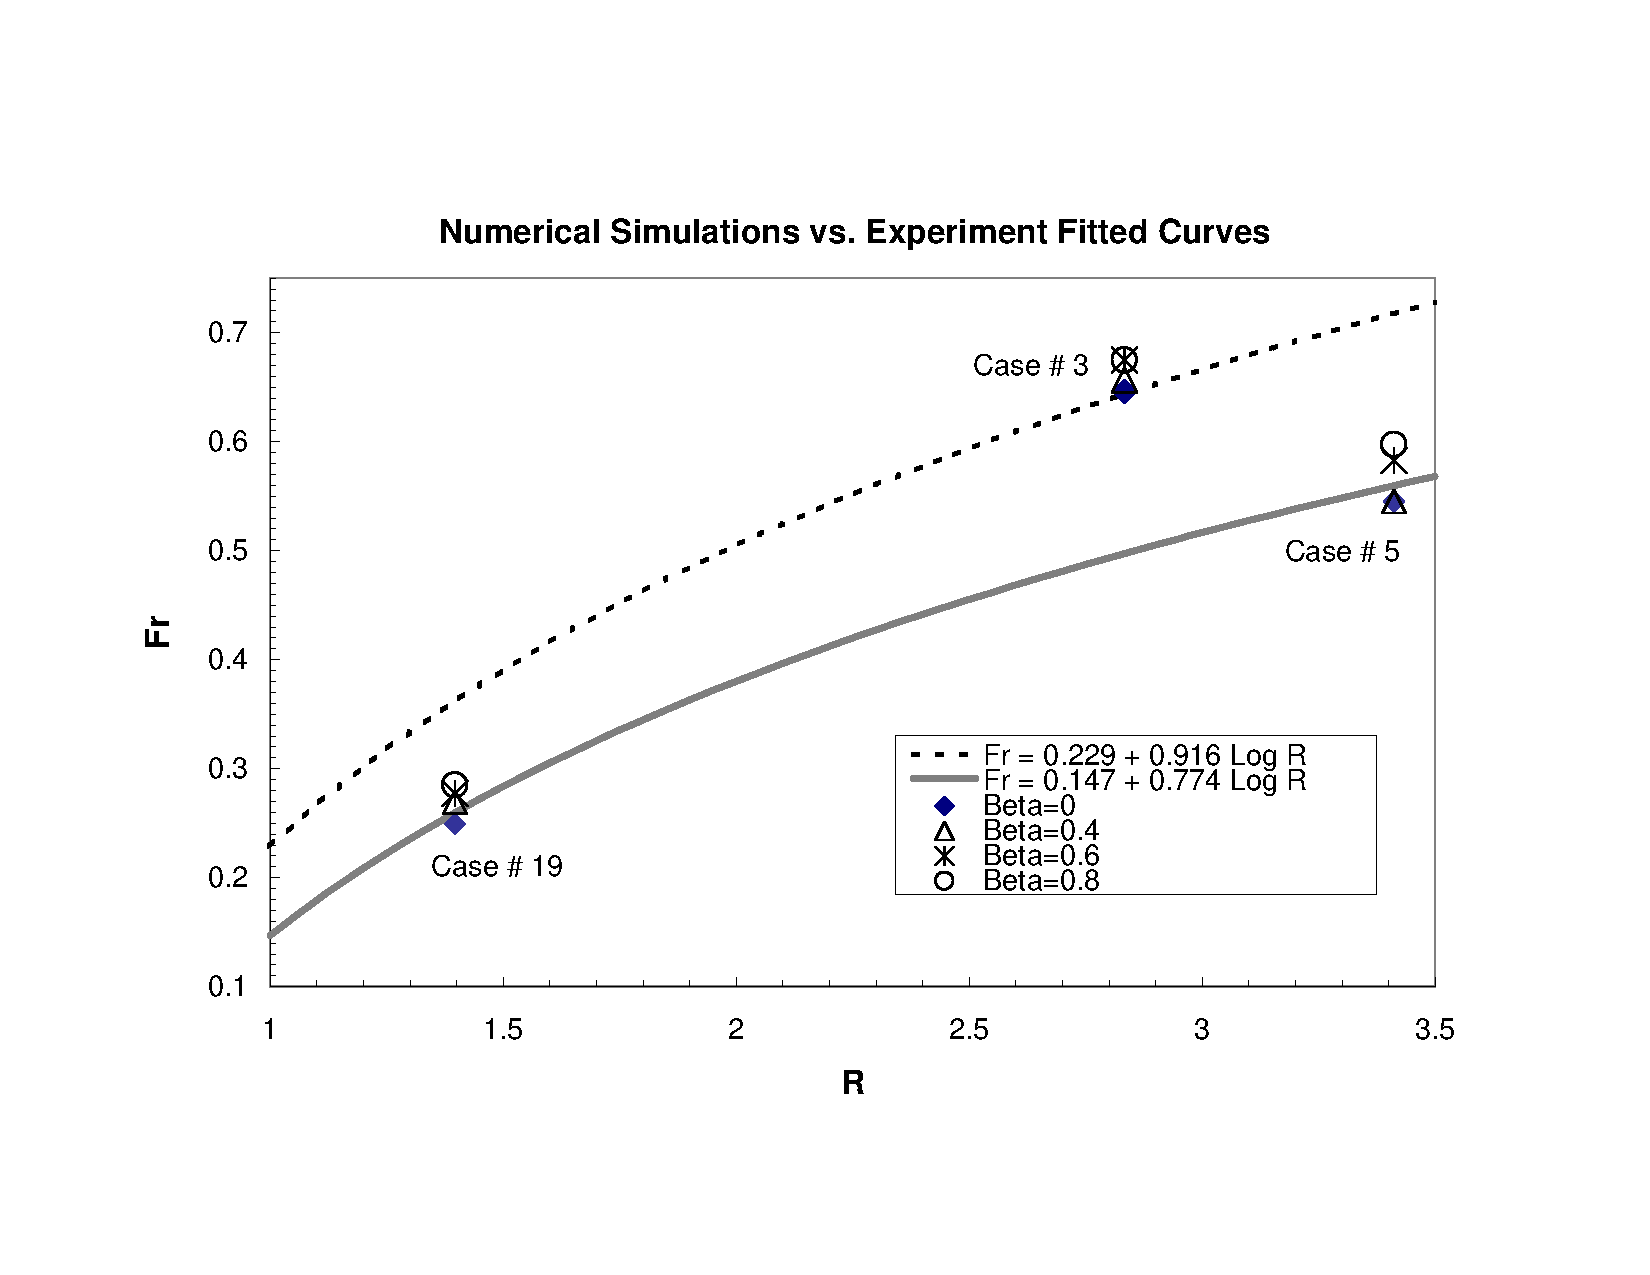
\includegraphics[width=5.5in]{../figures/Fr-R/Fr_R_060425.pdf}
\label{fig:GravityCurrents-Fr-R}
\caption{Numerical simulations with modified CIP method versus Experimental fitting Curves. The $\beta$ coefficient determines the weighting factor in the interpolation of the advection velocity. If $\beta = 0$, the advection velocity become the average of the neighboring velocities; if $\beta = 1$, then the advection velocity is the greater of the neighboring velocities.}
\end{figure}

\cp














%\abstract{
%The scalar transport is modeled by the advection of the mean velocity field and dispersion due to the velocity deviations. However, it has been known that the dispersion coefficient is more pronounced in the direction of the flow than the direction perpendicular to the flow. Therefore the use of dispersion coefficient involves the judgement of the flow direction; when the flow direction is not parallel to the established grid coordination, complicated procedure will also involved. Moreover, the dispersion coefficient is also depend on the field scale.
%We propose a method to evaluate the scalar transport as an simpler alternative to the traditional method.
%  for turbulent flow the advection term is difficult to be evaluated because of the velocity deviations. the usually evaluated after the velocity field computation has been done. However, for turbulent flow, the scalar transport is usually modeled by
%A modification of CIP method for staggered grid is proposed.
%}





% For two-dimensional case, the scalar variables are defined in the center of the cell, the x-direction velocity at the middle of vertical cell edges, and the z-direction velocity at the middle of the horizontal cell edges. Because the velocities in the x and z directions are not stored at the same locations as the scalar variables, an approximation equation for the advection velocities is proposed

\begin{comment}
The transport equation for some scalar $f$ without source term is:
\begin{equation}
\frac {\partial f}{\partial t} + u \frac {\partial f}{\partial x}+
w \frac {\partial f}{\partial z}=0 \label{equ:2Dfadvection}
\end{equation}

The CIP method solves the above equation by first using a cubic spline to construct a continuous scalar field $F$ between the grid points, and then carry this scalar field along with the advection velocities $u^a$ and $w^a$:
\begin{equation}
f(x, y, t+ \Delta t) = F(x-u^a \Delta t, y-w^a \Delta t, t)
\end{equation}



all the $C$ coefficients are computed from:
\begin{eqnarray}
 \frac{\partial F}{\partial x}_{(i,j)}=\frac{\partial f}{\partial
x}^*_{(i,j)}; \frac{\partial F}{\partial
x}_{(iup,j)}=\frac{\partial f^*}{\partial x}_{(iup,j)};
\frac{\partial F}{\partial x}_{(i,jup)}=\frac{\partial
f^*}{\partial x}_{(i,jup)}; \nonumber \\
 \frac{\partial F}{\partial y}_{(i,j)}=\frac{\partial f}{\partial
y}^*_{(i,j)}; \frac{\partial F}{\partial
y}_{(iup,j)}=\frac{\partial f^*}{\partial y}_{(iup,j)};
\frac{\partial F}{\partial y}_{(i,jup)}=\frac{\partial
f^*}{\partial y}_{(i,jup)}; \nonumber \\
F_{(i,j)}=f^*_{(i,j)}; F_{(iup,j)}=f^*_{(iup,j)};
F_{(i,jup)}=f^*_{(i,jup)}; F_{(iup,jup)}=f^*_{(iup,jup)};
\end{eqnarray}
\end{comment} 